\chapter{Бэкап и восстановление PostgreSQL}
\begin{epigraphs}
\qitem{Есть два типа администраторов~--- те, кто не делает бэкапы, и те, кто уже делает}{Народная мудрость}
\qitem{Если какая-нибудь неприятность может произойти, она случается.}{Закон Мэрфи}
\end{epigraphs}
\section{Введение}
Любой хороший сисадмин знает~--- бэкапы нужны всегда. 
На сколько бы надежна не казалась Ваша система, всегда может произойти случай, который был не учтен, и из-за которого 
могут быть потеряны данные.

Тоже самое касается и PostgreSQL баз данных. Бекапы должны быть! Посыпавшийся винчестер на сервере, ошибка в фаловой системе, 
ошибка в другой программе, которая перетерла весь каталог PostgreSQL и многое другое приведет только к плачевному результату.
И даже если у Вас репликация с множеством слейвов, 
это не означает, что система в безопасности~--- неверный запрос на мастер (DELETE, DROP), и у слейвов такая же порция данных 
(точнее их отсутствие). 

Существуют три принципиально различных подхода к резервному копированию данных PostgreSQL:
\begin{itemize}
\item SQL бэкап;
\item Бекап уровня файловой системы;
\item Непрерывное резервное копирование;
\end{itemize}
Каждый из этих подходов имеет свои сильные и слабые стороны.


\section{SQL бэкап}
Идея этого подхода в создании текстового файла с командами SQL. Такой файл можно передать обратно на сервер 
и воссоздать базу данных в том же состоянии, в котором она была во время бэкапа. 
У PostgreSQL для этого есть специальная утилита~--- pg\_dump. Пример использования pg\_dump:
\begin{lstlisting}[label=lst:backups1,caption=Создаем бэкап с помощью pg\_dump]
pg_dump dbname > outfile
\end{lstlisting}

Для восстановления такого бэкапа достаточно выполнить:
\begin{lstlisting}[label=lst:backups2,caption=Восстанавливаем бэкап]
psql dbname < infile
\end{lstlisting}

При этом базу данных <<dbname>> потребуется создать перед восстановлением. Также потребуется создать пользователей, 
которые имеют доступ к данным, которые восстанавливаются (это можно и не делать, но тогда просто в выводе восстановления будут ошибки).
Если нам требуется, чтобы восстановление прекратилось при возникновении ошибки, тогда потребуется восстанавливать бэкап таким способом:
\begin{lstlisting}[label=lst:backups3,caption=Восстанавливаем бэкап]
psql --set ON_ERROR_STOP=on dbname < infile
\end{lstlisting}

Также, можно делать бэкап и сразу восстанавливать его на другую базу:
\begin{lstlisting}[label=lst:backups4,caption=Бекап в другую БД]
pg_dump -h host1 dbname | psql -h host2 dbname
\end{lstlisting}

После восстановления бэкапа желательно запустить <<ANALYZE>>, чтобы оптимизатор запросов обновил статистику.

А что, если нужно сделать бэкап не одной базы данных, а всех, да и еще получить в бэкапе информацию про роли и таблицы? 
В таком случае у PostgreSQL есть утилита pg\_dumpall. pg\_dumpall используется для создания бэкапа данных всего кластера PostgreSQL:
\begin{lstlisting}[label=lst:backups5,caption=Бекап кластера PostgreSQL]
pg_dumpall > outfile
\end{lstlisting}

Для восстановления такого бэкапа достаточно выполнить от суперпользователя:
\begin{lstlisting}[label=lst:backups6,caption=Восстановления бэкапа PostgreSQL]
psql -f infile postgres
\end{lstlisting}

\subsection{SQL бэкап больших баз данных}
Некоторые операционные системы имеют ограничения на максимальный размер файла, что может вызывають проблемы при создании 
больших бэкапов через pg\_dump. К счастью, pg\_dump можете бэкапить в стандартный вывод. Так что можно использовать 
стандартные инструменты Unix, чтобы обойти эту проблему. Есть несколько возможных способов:
\begin{itemize}
\item \textbf{Использовать сжатие для бэкапа.} 

Можно использовать программу сжатия данных, например GZIP:
\begin{lstlisting}[label=lst:backups7,caption=Сжатие бэкапа PostgreSQL]
pg_dump dbname | gzip > filename.gz
\end{lstlisting}

Восстановление:
\begin{lstlisting}[label=lst:backups8,caption=Восстановление бэкапа PostgreSQL]
gunzip -c filename.gz | psql dbname
\end{lstlisting}
или
\begin{lstlisting}[label=lst:backups9,caption=Восстановление бэкапа PostgreSQL]
cat filename.gz | gunzip | psql dbname
\end{lstlisting}

\item \textbf{Использовать команду split.} 

Команда split позволяет разделить вывод в файлы меньшего размера, которые являются подходящими по размеру для файловой системы. 
Например, бэкап делится на куски по 1 мегабайту:
\begin{lstlisting}[label=lst:backups10,caption=Создание бэкапа PostgreSQL]
pg_dump dbname | split -b 1m - filename
\end{lstlisting}
Восстановление:
\begin{lstlisting}[label=lst:backups11,caption=Восстановление бэкапа PostgreSQL]
cat filename* | psql dbname
\end{lstlisting}

\item \textbf{Использовать пользовательский формат дампа pg\_dump}

PostgreSQL построен на системе с библиотекой сжатия Zlib, поэтому пользовательский формат бэкапа будет в сжатом виде. 
Это похоже на метод с импользованием GZIP, но он имеет дополнительное преимущество~--- таблицы могут быть восстановлены выборочно:
\begin{lstlisting}[label=lst:backups12,caption=Создание бэкапа PostgreSQL]
pg_dump -Fc dbname > filename
\end{lstlisting}
Через psql такой бэкап не восстановить, но для этого есть утилита pg\_restore:
\begin{lstlisting}[label=lst:backups13,caption=Восстановление бэкапа PostgreSQL]
pg_restore -d dbname filename
\end{lstlisting}

\end{itemize}

При слишком большой базе данных, вариант с командой split нужно комбинировать с сжатием данных.


\section{Бекап уровня файловой системы}
Альтернативный метод резервного копирования заключается в непосредственном копировании файлов, 
которые PostgreSQL использует для хранения данных в базе данных. Например:
\begin{lstlisting}[label=lst:backups14,caption=Бэкап PostgreSQL файлов]
tar -cf backup.tar /usr/local/pgsql/data
\end{lstlisting}

Но есть два ограничения, которые делает этот метод нецелесообразным, или, по крайней мере, уступающим SQL бэкапу:
\begin{itemize}
\item PostgreSQL база данных должна быть остановленна, для того, чтобы получить актуальный бэкап 
(PostgreSQL держит множество обьектов в памяти, буферизация файловой системы). Излишне говорить, 
что во время восстановления такого бэкапа потребуется также остановить PostgreSQL.
\item Не получится востановить только определенные данные с такого бэкапа.
\end{itemize}

Как альтернатива, можно делать снимки (snapshot) файлов системы (папки с файлами PostgreSQL). В таком случае останавливать PostgreSQL 
не требуется. Однако, резервная копия, созданная таким образом, сохраняет файлы базы данных в состоянии, как если бы сервер базы данных 
был неправильно остановлен. Поэтому при запуске PostgreSQL из резервной копии, он будет думать, что предыдущий экземпляр 
сервера вышел из строя и повторит журнала WAL. Это не проблема, просто надо знать про это (и не забыть включить WAL файлы 
в резервную копию). Также, если файловая система PostgreSQL распределена по разным файловым система, то такой метод бэкапа 
будет очень не надежным~--- снимки файлов системы должны быть сделаны одновременно(!!!). Почитайте документацию файловой 
системы очень внимательно, прежде чем доверять снимкам файлов системы в таких ситуациях.

Также возможен вариант с использованием rsync. Первым запуском rsync мы копируем основные файлы с директории PostgreSQL 
(PostgreSQL при этом продолжает работу). После этого 
мы останавливаем PostgreSQL и запускаем повторно rsync. Второй запуск rsync пройдет гораздо быстрее, чем первый, 
потому что будет передавать относительно небольшой размер данных, 
и конечный результат будет соответствовать остановленной СУБД. 
Этот метод позволяет делать бекап уровня файловой системы с минимальным временем простоя.

\section{Непрерывное резервное копирование}
PostgreSQL поддерживает упреждаюшию запись логов (Write Ahead Log, WAL) в pg\_xlog директорию, которая находится в директории 
данных СУБД. 
В логи пишутся все изменения сделаные с данными в СУБД. Этот журнал существует прежде всего для безопасности во 
время краха PostgreSQL: если происходят сбои в системе, базы данных могут быть восстановлены с помощью <<перезапуска>> этого 
журнала. Тем не менее, существование журнала делает возможным использование третью стратегии для резервного копирования 
баз данных: мы можем объединить бекап уровня файловой системы с резервной копией WAL файлов. Если требуется восстановить такой бэкап, то 
мы восстановливаем файлы резервной копии файловой системы, а затем <<перезапускаем>> с резервной копии файлов WAL для приведения 
системы к актуальному состоянию. Этот подход является более сложным для администрирования, чем любой из предыдущих подходов, 
но он имеет некоторые преимущества:
\begin{itemize}
\item Не нужно согласовывать файлы резервной копии системы. Любая внутренняя противоречивость в резервной копии будет исправлена 
путем преобразования журнала (не отличается от того, что происходит во время восстановления после сбоя). 
\item Восстановление состояния сервера для определенного момента времени.
\item Если мы постоянно будем <<скармливать>> файлы WAL на другую машину, которая была загружена с тех же файлов резервной базы, 
то у нас будет резервный сервер PostgreSQL всегда в актуальном состоянии (создание сервера горячего резерва).
\end{itemize}

Как и бэкап файловой системы, этот метод может поддерживать только восстановление всей базы данных кластера. Кроме того, он требует 
много места для хранения WAL файлов.

\subsection{Настройка}
Первый шаг~--- активировать архивирование. Эта процедура будет копировать WAL файлы в архивный каталог из 
стандартного каталога pg\_xlog. Это делается в файле postgresql.conf:
\begin{lstlisting}[label=lst:backups15,caption=Настройка архивирования]
archive_mode = on # enable archiving
archive_command = 'cp -v %p /data/pgsql/archives/%f'
archive_timeout = 300 # timeout to close buffers
\end{lstlisting}

После этого необходимо перенести файлы (в порядке их появления) в архивный каталог. 
Для этого можно использовать функцию rsync.
Можно поставить функцию в список задач крона и, таким образом, файлы могут автоматически перемещаться между 
хостми каждые несколько минут.
\begin{lstlisting}[label=lst:backups16,caption=Копирование WAL файлов на другой хост]
rsync -avz --delete prod1:/data/pgsql/archives/ \
/data/pgsql/archives/ > /dev/null
\end{lstlisting}

В конце, необходимо скопировать файлы в каталог pg\_xlog на сервере PostgreSQL (он должен быть в режиме восстановления). 
Для этого создается в каталоге данных PostgreSQL создать файл recovery.conf с заданной командой копирования 
файлов из архива в нужную директорию:
\begin{lstlisting}[label=lst:backups17,caption=recovery.conf]
restore_command = 'cp /data/pgsql/archives/%f "%p"'
\end{lstlisting}

Документация PostgreSQL предлагает хорошее описание настройки непрерывного копирования, поэтому я не углублялся в детали 
(например, как перенести директорию СУБД с одного сервера на другой, какие могут быть проблемы). Более подробно вы 
можете почитать по этой ссылке http://www.postgresql.org/docs/9.0/static/continuous-archiving.html.

\section{Утилиты для непрерывного резервного копирования}

\subsection{WAL-E}

\href{https://github.com/wal-e/wal-e}{WAL-E} предназначенная для непрерывной архивации PostgreSQL WAL-logs в Amazon S3 или Windows Azure (начиная с версии 0.7) и управления использованием \lstinline!pg_start_backup! и \lstinline!pg_stop_backup!. Утилита написана на Python и разработана в компании \href{http://www.heroku.com/}{Heroku}, где её активно используют.


\subsubsection{Установка}

У WAL-E есть пару зависимостей: lzop, psql, pv (в старых версиях используется mbuffer), python 2.6+ и несколько python библиотек (gevent >= 0.13, boto >= 2.0, azure). Также для удобства настроек переменных среды устанавливается daemontools. На Ubuntu это можно все поставить одной командой:

\begin{lstlisting}[language=Bash,label=lst:wal-e1,caption=Установка зависимостей для WAL-E]
$ aptitude install git-core python-dev python-setuptools python-pip build-essential libevent-dev lzop pv daemontools daemontools-run
\end{lstlisting}

Теперь установим WAL-E:

\begin{lstlisting}[language=Bash,label=lst:wal-e2,caption=Установка WAL-E]
$ pip install https://github.com/wal-e/wal-e/archive/v1.0.1.tar.gz
\end{lstlisting}

После успешной установки можно начать работать с WAL-E.

\subsubsection{Настройка и работа}

Как уже писалось, WAL-E сливает все данные в AWS S3, поэтому нам потребуются <<Access Key ID>>, <<Secret Access Key>> и <<AWS Region>> (эти данные можно найти в акаунте Amazon AWS). Команда для загрузки бэкапа всей базы данных в S3:

\begin{lstlisting}[language=Bash,label=lst:wal-e3,caption=Загрузка бэкапа всей базы данных в S3]
AWS_REGION=... AWS_SECRET_ACCESS_KEY=... wal-e                     \
  -k AWS_ACCESS_KEY_ID                                \
  --s3-prefix=s3://some-bucket/directory/or/whatever  \
  backup-push /var/lib/postgresql/9.2/main
\end{lstlisting}

Где \lstinline!s3-prefix!~--- URL, который содержит имя S3 бакета (bucket) и путь к папке, куда следует складывать резервные копии. Команда для загрузки WAL-логов на S3:

\begin{lstlisting}[language=Bash,label=lst:wal-e4,caption=Загрузка WAL-логов на S3]
AWS_REGION=... AWS_SECRET_ACCESS_KEY=... wal-e                     \
  -k AWS_ACCESS_KEY_ID                                \
  --s3-prefix=s3://some-bucket/directory/or/whatever  \
  wal-push /var/lib/postgresql/9.2/main/pg_xlog/WAL_SEGMENT_LONG_HEX
\end{lstlisting}

Для управления этими переменными окружения можно использовать команду \lstinline!envdir! (идет в поставке с \lstinline!daemontools!). Для этого создадим \lstinline!envdir! каталог:

\begin{lstlisting}[language=Bash,label=lst:wal-e5,caption=WAL-E с envdir]
$ mkdir -p /etc/wal-e.d/env
$ echo "aws_region" > /etc/wal-e.d/env/AWS_REGION
$ echo "secret-key" > /etc/wal-e.d/env/AWS_SECRET_ACCESS_KEY
$ echo "access-key" > /etc/wal-e.d/env/AWS_ACCESS_KEY_ID
$ echo 's3://some-bucket/directory/or/whatever' > /etc/wal-e.d/env/WALE_S3_PREFIX
$ chown -R root:postgres /etc/wal-e.d
\end{lstlisting}

После создания данного каталога появляется возможность запускать WAL-E команды гораздо проще и с меньшим риском случайного использования некорректных значений:

\begin{lstlisting}[language=Bash,label=lst:wal-e6,caption=WAL-E с envdir]
$ envdir /etc/wal-e.d/env wal-e backup-push ...
$ envdir /etc/wal-e.d/env wal-e wal-push ...
\end{lstlisting}

Теперь настроим PostgreSQL для сбрасывания WAL-логов в S3 c помощью WAL-E. Отредактируем \lstinline!postgresql.conf!:

\begin{lstlisting}[language=Bash,label=lst:wal-e7,caption=Настройка PostgreSQL]
wal_level = hot_standby # или archive, если PostgreSQL < 9.0
archive_mode = on
archive_command = 'envdir /etc/wal-e.d/env /usr/local/bin/wal-e wal-push %p'
archive_timeout = 60
\end{lstlisting}

Лучше указать полный путь к WAL-E (можно узнать командой \lstinline!which wal-e!), поскольку PostgreSQL может его не найти. После этого нужно перегрузить PostgreSQL. В логах базы вы должны увидеть что-то подобное:

\begin{lstlisting}[language=Bash,label=lst:wal-e8,caption=Логи PostgreSQL]
2016-11-07 14:52:19 UTC LOG:  database system was shut down at 2016-11-07 14:51:40 UTC
2016-11-07 14:52:19 UTC LOG:  database system is ready to accept connections
2016-11-07 14:52:19 UTC LOG:  autovacuum launcher started
2016-11-07T14:52:19.784+00 pid=7653 wal_e.worker.s3_worker INFO     MSG: begin archiving a file
        DETAIL: Uploading "pg_xlog/000000010000000000000001" to "s3://cleverdb-pg-backups/pg/wal_005/000000010000000000000001.lzo".
2016-11-07 14:52:19 UTC LOG:  incomplete startup packet
2016-11-07T14:52:28.234+00 pid=7653 wal_e.worker.s3_worker INFO     MSG: completed archiving to a file
        DETAIL: Archiving to "s3://cleverdb-pg-backups/pg/wal_005/000000010000000000000001.lzo" complete at 21583.3KiB/s.
2016-11-07T14:52:28.341+00 pid=7697 wal_e.worker.s3_worker INFO     MSG: begin archiving a file
        DETAIL: Uploading "pg_xlog/000000010000000000000002.00000020.backup" to "s3://cleverdb-pg-backups/pg/wal_005/000000010000000000000002.00000020.backup.lzo".
2016-11-07T14:52:34.027+00 pid=7697 wal_e.worker.s3_worker INFO     MSG: completed archiving to a file
        DETAIL: Archiving to "s3://cleverdb-pg-backups/pg/wal_005/000000010000000000000002.00000020.backup.lzo" complete at 00KiB/s.
2016-11-07T14:52:34.187+00 pid=7711 wal_e.worker.s3_worker INFO     MSG: begin archiving a file
        DETAIL: Uploading "pg_xlog/000000010000000000000002" to "s3://cleverdb-pg-backups/pg/wal_005/000000010000000000000002.lzo".
2016-11-07T14:52:40.232+00 pid=7711 wal_e.worker.s3_worker INFO     MSG: completed archiving to a file
        DETAIL: Archiving to "s3://cleverdb-pg-backups/pg/wal_005/000000010000000000000002.lzo" complete at 2466.67KiB/s.
\end{lstlisting}

Если ничего похожего в логах не видно, тогда нужно смотреть что за ошибка появляется и исправлять её. Для того, чтобы бэкапить всю базу достаточно выполнить данную команду:

\begin{lstlisting}[language=Bash,label=lst:wal-e9,caption=Загрузка бэкапа всей базы данных в S3]
$ envdir /etc/wal-e.d/env wal-e backup-push /var/lib/postgresql/9.2/main
2016-11-07T14:49:26.174+00 pid=7493 wal_e.operator.s3_operator INFO     MSG: start upload postgres version metadata
        DETAIL: Uploading to s3://cleverdb-pg-backups/pg/basebackups_005/base_000000010000000000000006_00000032/extended_version.txt.
2016-11-07T14:49:32.783+00 pid=7493 wal_e.operator.s3_operator INFO     MSG: postgres version metadata upload complete
2016-11-07T14:49:32.859+00 pid=7493 wal_e.worker.s3_worker INFO     MSG: beginning volume compression
        DETAIL: Building volume 0.
...
HINT:  Check that your archive_command is executing properly.  pg_stop_backup can be canceled safely, but the database backup will not be usable without all the WAL segments.
NOTICE:  pg_stop_backup complete, all required WAL segments have been archived
\end{lstlisting}

\begin{figure}[h!]
  \center{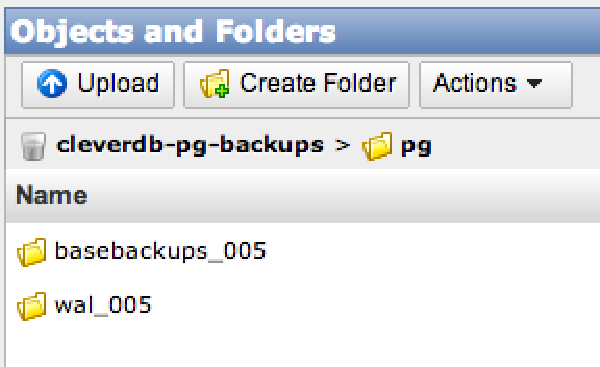
\includegraphics[width=0.6\textwidth]{wale1.pdf}}
  \caption{Папка бэкапов на S3}
  \label{fig:wal-e1}
\end{figure}

\begin{figure}[h!]
  \center{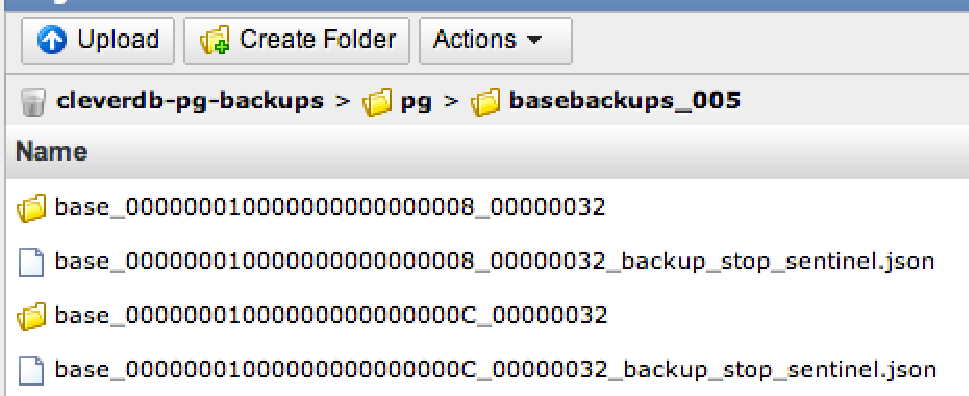
\includegraphics[width=0.6\textwidth]{wale2.pdf}}
  \caption{Папка бэкапов базы на S3}
  \label{fig:wal-e2}
\end{figure}

\begin{figure}[h!]
  \center{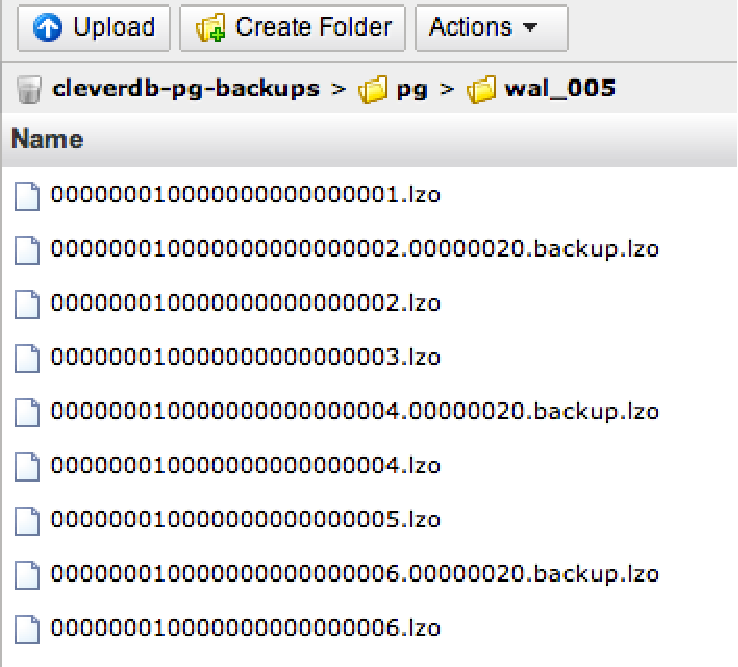
\includegraphics[width=0.6\textwidth]{wale3.pdf}}
  \caption{Папка WAL-логов на S3}
  \label{fig:wal-e3}
\end{figure}

Данный бэкап лучше делать раз в сутки (например, добавить в \lstinline!crontab!). На рис~\ref{fig:wal-e1}-\ref{fig:wal-e3} видно как хранятся бэкапы на S3. Все бэкапы сжаты через \href{http://en.wikipedia.org/wiki/Lzop}{lzop}. Данный алгоритм сжимает хуже чем gzip, но скорость сжатия намного быстрее (приблизительно 25 Мб/сек используя 5\% ЦПУ). Чтобы уменьшить нагрузку на чтение с жесткого диска бэкапы отправляются через \lstinline!pv! утилиту (опцией \lstinline!cluster-read-rate-limit! можно ограничить скорость чтения, если это требуется).

Теперь перейдем к восстановлению данных. Для восстановления базы из резервной копии используется \lstinline!backup-fetch! команда:

\begin{lstlisting}[language=Bash,label=lst:wal-e10,caption=Восстановление бэкапа базы из S3]
$ sudo -u postgres bash -c "envdir /etc/wal-e.d/env wal-e  --s3-prefix=s3://some-bucket/directory/or/whatever backup-fetch /var/lib/postgresql/9.2/main LATEST"
\end{lstlisting}

Где \lstinline!LATEST! означает восстановится из последнего актуального бэкапа (PostgreSQL в это время должен быть остановлен). Для восстановления из более поздней резервной копии:

\begin{lstlisting}[language=Bash,label=lst:wal-e11,caption=Восстановление из поздней резервной копии]
$ sudo -u postgres bash -c "envdir /etc/wal-e.d/env wal-e  --s3-prefix=s3://some-bucket/directory/or/whatever backup-fetch /var/lib/postgresql/9.2/main base_LONGWALNUMBER_POSITION_NUMBER"
\end{lstlisting}

Для получения списка доступных резервных копий есть команда \lstinline!backup-list!:

\begin{lstlisting}[language=Bash,label=lst:wal-e12,caption=Список резервных копий]
$ envdir /etc/wal-e.d/env wal-e backup-list
name	last_modified	expanded_size_bytes	wal_segment_backup_start	wal_segment_offset_backup_start	wal_segment_backup_stop	wal_segment_offset_backup_stop
base_000000010000000000000008_00000032	2016-11-07T14:00:07.000Z		000000010000000000000008	00000032
base_00000001000000000000000C_00000032	2016-11-08T15:00:08.000Z		00000001000000000000000C	00000032
\end{lstlisting}

После завершения работы с основной резервной копией для полного восстановления нужно считать WAL-логи (чтобы данные обновились до последнего состояния). Для этого используется \lstinline!recovery.conf!:

\begin{lstlisting}[language=Bash,label=lst:wal-e13,caption=recovery.conf]
restore_command = 'envdir /etc/wal-e.d/env /usr/local/bin/wal-e wal-fetch "%f" "%p"'
\end{lstlisting}

После создания этого файла нужно запустить PostgreSQL. Через небольшой интервал времени база станет полностью восстановленной.

Для удаления старых резервных копий (или вообще всех) используется команда \lstinline!delete!:

\begin{lstlisting}[language=Bash,label=lst:wal-e14,caption=Удаление резервных копий]
# удаления старых бэкапов старше base_00000004000002DF000000A6_03626144
$ envdir /etc/wal-e.d/env wal-e delete --confirm before base_00000004000002DF000000A6_03626144
# удаления всех бэкапов
$ envdir /etc/wal-e.d/env wal-e delete --confirm everything
# удалить все старше последних 20 бэкапов
$ envdir /etc/wal-e.d/env wal-e delete --confirm retain 20
\end{lstlisting}

Без опции \lstinline!--confirm! команды будут запускаться и показывать, что будет удаляться, но фактического удаления не будет производиться (dry run).

\subsubsection{Заключение}

WAL-E помогает автоматизировать сбор резервных копий с PostgreSQL и хранить их в достаточно дешевом и надежном хранилище~--- Amazon S3 или Windows Azure.

\subsection{Barman}
\textbf{Ссылка}: \href{http://www.pgbarman.org/}{www.pgbarman.org}

Barman, как и WAL-E, позволяет создать систему для бэкапа и восстановления PostgreSQL на основе непрерывного бэкапа.

\subsubsection{Установка}



\section{Заключение}
В любом случае, усилия и время, затраченные на создание оптимальной системы создания бэкапов, будут оправданы. 
Невозможно предугадать когда произойдут проблемы с базой данных, поэтому бэкапы должны быть настроены для PostgreSQL 
(особенно, если это продакшн система).